\section{Empirical Evaluation}

\begin{figure}[t]
\centering
\subfigure{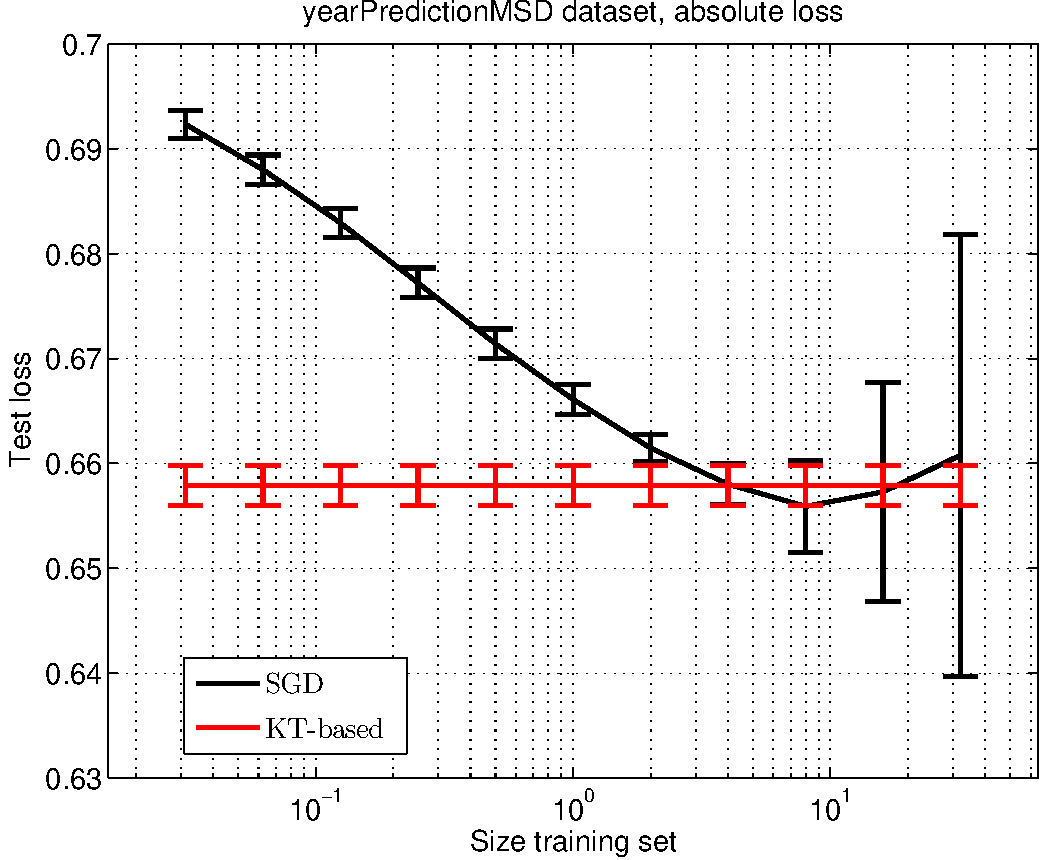
\includegraphics[width=0.32\textwidth]{figs/yearPredictionMSD_kt_train_test-crop.pdf}}
\subfigure{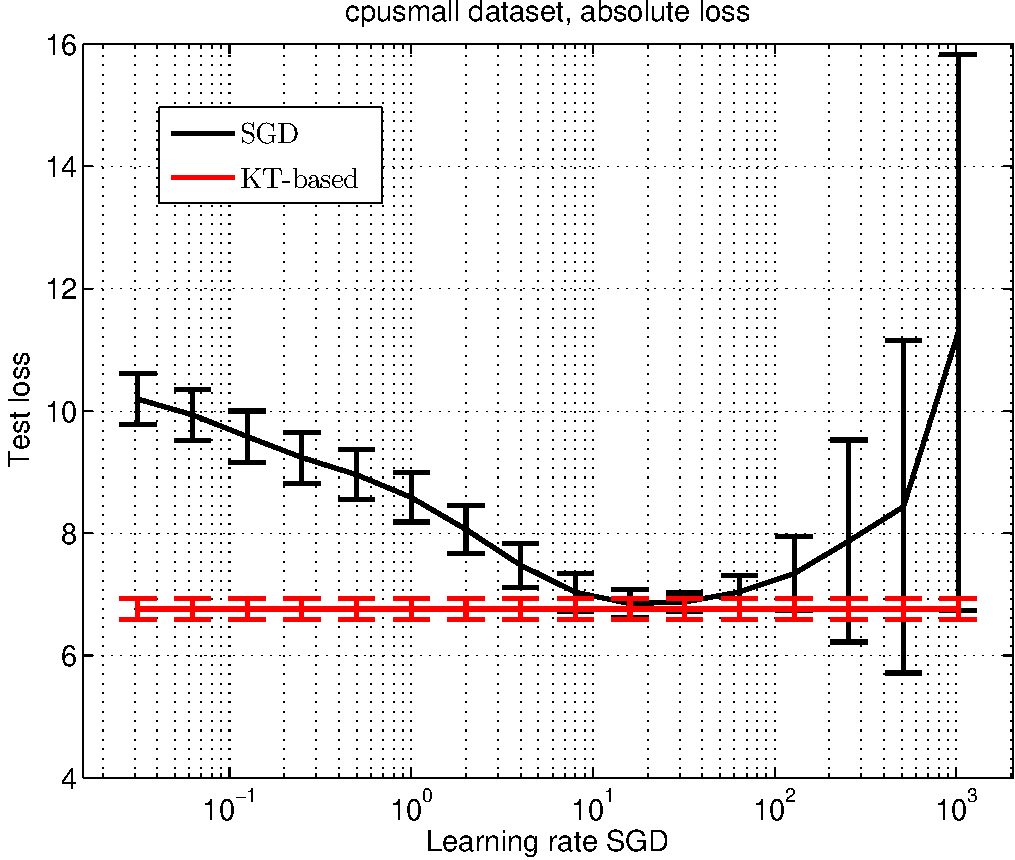
\includegraphics[width=0.32\textwidth]{figs/cpusmall_kt_train_test-crop.pdf}}
\subfigure{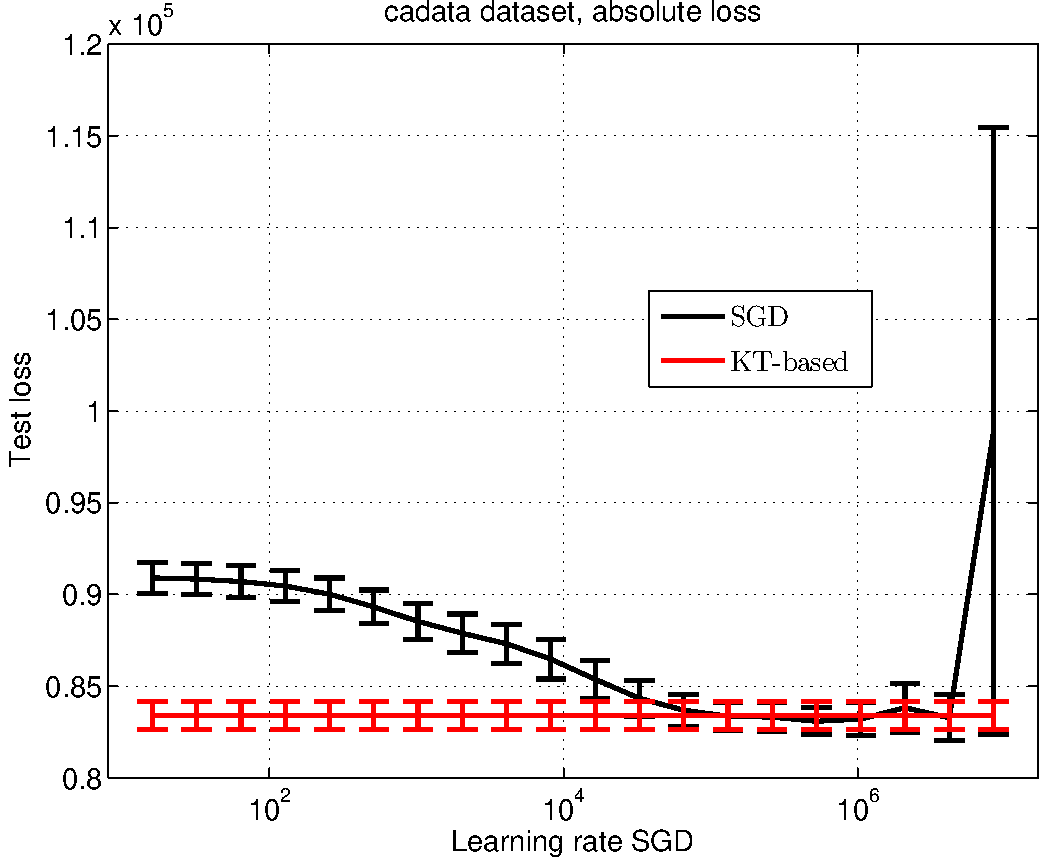
\includegraphics[width=0.32\textwidth]{figs/cadata_kt_train_test-crop.pdf}}
\caption{\footnotesize{Test loss versus learning rate parameter of \ac{SGD} (in log scale), compared with the parameter-free Algorithm~\ref{algorithm:averaged-olo}.}}
\label{figure:experiments-olo}
\end{figure}

We have also run a small empirical evaluation to show that the theoretical
difference between classic learning algorithms and parameter-free ones is real
and not just theoretical. In Figure~\ref{figure:experiments-olo}, we have used
three regression datasets\footnote{Datasets available at
\url{https://www.csie.ntu.edu.tw/~cjlin/libsvmtools/datasets/}.}, and solved
the \ac{OCO} problem through \ac{OLO}. In all the three cases, we have used the
absolute loss and normalized the input vectors to have L2 norm equal to 1. 

The dataset were split in two parts: 75\% training set and the remaining as test set. The training is done through one pass over the training set and the final classifier is evaluated on the test set. We used 5 different splits of training/test and we report average and standard deviations. 

We have run \ac{SGD} with different learning rates and shown the performance of its last solution on the test set. For Algorithm~\ref{algorithm:averaged-olo}, we do not have any parameter to tune so we just plot its test set performance as a line.

From the empirical results, it is clear that the optimal learning rate is completely
data-dependent. It is also interesting to note how the performance of \ac{SGD} becomes very unstable with large learning rates. Yet \emph{our parameter-free algorithm has a performance very close
to the unknown optimal tuning of the learning rate of \ac{SGD}}.
